\hypertarget{Entrypoint_8h}{}\section{engine/src/core/\+Entrypoint.h File Reference}
\label{Entrypoint_8h}\index{engine/src/core/\+Entrypoint.\+h@{engine/src/core/\+Entrypoint.\+h}}


The entrypoint into the engine.  


{\ttfamily \#include \char`\"{}core/\+Application.\+h\char`\"{}}\newline
{\ttfamily \#include \char`\"{}core/\+Log.\+h\char`\"{}}\newline
Include dependency graph for Entrypoint.\+h\+:
\nopagebreak
\begin{figure}[H]
\begin{center}
\leavevmode
\includegraphics[width=350pt]{Entrypoint_8h__incl}
\end{center}
\end{figure}
This graph shows which files directly or indirectly include this file\+:
\nopagebreak
\begin{figure}[H]
\begin{center}
\leavevmode
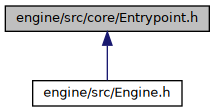
\includegraphics[width=219pt]{Entrypoint_8h__dep__incl}
\end{center}
\end{figure}


\subsection{Detailed Description}
The entrypoint into the engine. 

It defines the Create\+Application function as an external function that is to be implemented in the application. 